\begin{frame}[fragile]{Visualização da união de árvores}

    \begin{figure}
        \centering

        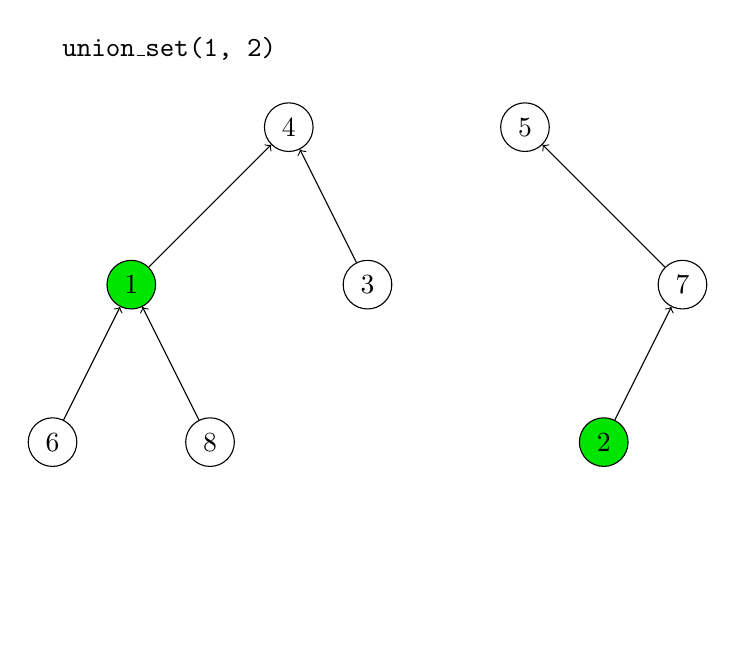
\begin{tikzpicture}
            \node[anchor=west] at (0, 6) { \tt union\_set(1, 2) };

            \node[draw,circle] (A) at (3, 5) { 4 };
            \node[draw,circle,fill=green!90!black] (B) at (1, 3) { 1 };
            \node[draw,circle] (C) at (4, 3) { 3 };
            \node[draw,circle] (D) at (0, 1) { 6 };
            \node[draw,circle] (E) at (2, 1) { 8 };

            \node[draw,circle] (F) at (6, 5) { 5 };
            \node[draw,circle] (G) at (8, 3) { 7 };
            \node[draw,circle,fill=green!90!black] (H) at (7, 1) { 2 };
            \node[draw,circle,opacity=0] (I) at (7, -1) { 2 };

            \draw[->] (B) edge (A);
            \draw[->] (C) edge (A);
            \draw[->] (D) edge (B);
            \draw[->] (E) edge (B);

            \draw[->] (G) edge (F);
            \draw[->] (H) edge (G);

        \end{tikzpicture}

    \end{figure}

\end{frame}

\begin{frame}[fragile]{Visualização da união de árvores}

    \begin{figure}
        \centering

        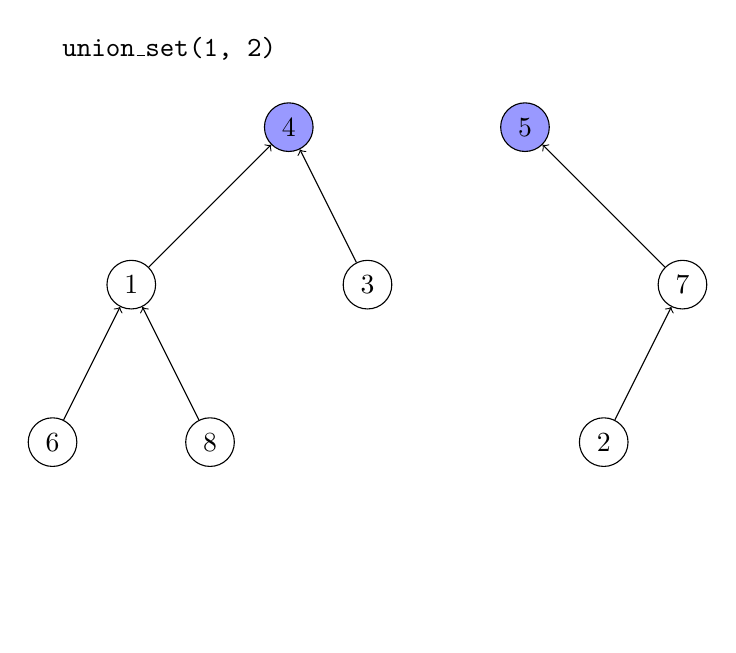
\begin{tikzpicture}
            \node[anchor=west] at (0, 6) { \tt union\_set(1, 2) };

            \node[draw,circle,fill=blue!40] (A) at (3, 5) { 4 };
            \node[draw,circle] (B) at (1, 3) { 1 };
            \node[draw,circle] (C) at (4, 3) { 3 };
            \node[draw,circle] (D) at (0, 1) { 6 };
            \node[draw,circle] (E) at (2, 1) { 8 };

            \node[draw,circle,fill=blue!40] (F) at (6, 5) { 5 };
            \node[draw,circle] (G) at (8, 3) { 7 };
            \node[draw,circle] (H) at (7, 1) { 2 };
            \node[draw,circle,opacity=0] (I) at (7, -1) { 2 };

            \draw[->] (B) edge (A);
            \draw[->] (C) edge (A);
            \draw[->] (D) edge (B);
            \draw[->] (E) edge (B);

            \draw[->] (G) edge (F);
            \draw[->] (H) edge (G);

        \end{tikzpicture}

    \end{figure}

\end{frame}

\begin{frame}[fragile]{Visualização da união de árvores}

    \begin{figure}
        \centering

        \begin{tikzpicture}
            \node[anchor=west] at (0, 6) { \tt union\_set(1, 2) };

            \node[draw,circle] (A) at (3, 5) { 4 };
            \node[draw,circle] (B) at (1, 3) { 1 };
            \node[draw,circle] (C) at (4, 3) { 3 };
            \node[draw,circle] (D) at (0, 1) { 6 };
            \node[draw,circle] (E) at (2, 1) { 8 };

            \node[draw,circle] (F) at (6, 3) { 5 };
            \node[draw,circle] (G) at (8, 1) { 7 };
            \node[draw,circle] (H) at (7, -1) { 2 };
            \node[draw,circle,opacity=0] (I) at (7, -1) { 2 };

            \draw[->] (B) edge (A);
            \draw[->] (C) edge (A);
            \draw[->] (D) edge (B);
            \draw[->] (E) edge (B);

            \draw[->] (F) edge (A);
            \draw[->] (G) edge (F);
            \draw[->] (H) edge (G);

        \end{tikzpicture}

    \end{figure}

\end{frame}


